\chapter{简约波矢$\vec k$的物理意义和$\vec k$空间积分}
\section{简约波矢$\vec k$}
对于周期体系,波函数满足周期性边界条件(也称\textrm{Born-Von Karman}条件),即:~
\begin{equation}
  \left\{
  \begin{aligned}
     \psi(\vec r+N_1\vec{\mathbf a}_1)&=\psi(\vec r)\\
     \psi(\vec r+N_2\vec{\mathbf a}_2)&=\psi(\vec r)\\
     \psi(\vec r+N_3\vec{\mathbf a}_3)&=\psi(\vec r)\\
   \end{aligned}\right.
  \label{eq:solid-31}
\end{equation}
其中$\vec{\mathbf a}_i(i=1,2,3)$是\textrm{Bravais}格子的三个基矢,$N_1$、$N_2$、$N_3$分别是沿着基矢$\vec{\mathbf a}_1$、$\vec{\mathbf a}_2$、$\vec{\mathbf a}_3$方向的原胞数,$N=N_1N_2N_3$是晶体中的原胞总数,同时波函数服从由\textrm{Bloch}定理,%将式\eqref{eq:bloch}代入\eqref{eq:solid-31}得
\begin{equation}
	\psi(\vec r+N_i\vec{\mathbf a}_i)=\mathrm{e}^{\mathrm{i}N_i\vec k\cdot\vec{\mathbf a}_i}\psi(\vec r),\quad i=1,2,3
  \label{eq:solid-32}
\end{equation}
因此有等式
\begin{equation}
	\mathrm{e}^{\mathrm{i}N_i\vec k\cdot\vec{\mathbf a}_i}=1,
	\label{eq:solid-33}
\end{equation}
%\begin{equation}
%  e^{iN_i\vec k\cdot\vec{\mathbf a}_i}=1,\quad i=1,2,3
%  \label{eq:solid-33}
%\end{equation}
%或者等价地
%\begin{equation}
%  N_i\vec k\cdot\vec{\mathbf a}_i=2\pi l_i,\quad l_i\mbox{为整数},\quad i=1,2,3
%  \label{eq:solid-34}
%\end{equation}
不难看出,波矢$\vec k$%(相应的本征值$\lambda_{\vec R_n}$)
的取值将受到限制,%根据等式\eqref{eq:solid-33},
并且$\vec k$可用相应的倒格子基矢$\vec{\mathbf b}_i(i=1,2,3)$表示,倒格子基矢围成空间中的波矢称为简约波矢。%即
%\begin{equation}
%  \vec k=k_1\vec{\mathbf b}_1+k_2\vec{\mathbf b}_2+k_3\vec{\mathbf b}_3
%  \label{eq:solid-35}
%\end{equation}
%代入式\eqref{eq:solid-34},并
根据正格子和倒格子的正交关系%式\eqref{eq:solid-12}
$\vec{\mathbf a}_i\cdot\vec{\mathbf b}_j=2\pi\delta_{ij}$,有
\begin{equation}
  \vec k=\dfrac{l_1}{N_1}\vec{\mathbf b}_1+\dfrac{l_2}{N_2}\vec{\mathbf b}_2+\dfrac{l_3}{N_3}\vec{\mathbf b}_3
  \label{eq:solid-36}
\end{equation}
简约波矢$\vec k$可以看成是倒格子空间中以$\dfrac{\vec{\mathbf b}_i}{N_i}(i=1,2,3)$为基矢的\textrm{Bravais}格子的格矢。
%每个许可的$\vec k$值由上述\textrm{Bravais}格子的格点表示,由
倒格子空间中由$\vec k$点围成的最小重复单元的体积为
\begin{equation}
  \Delta\vec k=\dfrac{\vec{\mathbf b}_1}{N_1}\cdot\biggl(\dfrac{\vec{\mathbf b}_2}{N_2}\times\dfrac{\vec{\mathbf b}_3}{N_3}\biggr)=\dfrac1N\vec{\mathbf b}_1\cdot(\vec{\mathbf b}_2\times\vec{\mathbf b}_3)
  \label{eq:solid-37}
\end{equation}
$\vec{\mathbf b}_1\cdot(\vec{\mathbf b}_2\times\vec{\mathbf b}_3)$是倒格子原胞的体积,因此倒格子原胞中许可简约波矢的数目等于实空间中晶体的总的原胞数目。

倒格子原胞体积为$\dfrac{(2\pi)^3}{\Omega_0}$,%式\eqref{eq:solid-14},
$\Omega_0$是正格子的原胞体积,$N\Omega_0=V$。波矢$\vec k$是体系运动状态的标志(特别地,对于用平面波描述的自由电子,$\hbar\vec k$是电子的动量\cite{Yanshousheng}),因此,在倒格子空间中的态密度
\begin{equation}
  \dfrac1{\Delta\vec k}=\dfrac V{8\pi^3}
  \label{eq:solid-38}
\end{equation}

对于一般周期式中的\textrm{Bloch}电子,简约波矢$\vec k$并不正比于电子的动量。动量算符$p=-\mathrm{i}\hbar\nabla$作用于\textrm{Bloch}波函数%(式\eqref{eq:blochpw})上,
\begin{equation}
  \begin{split}
	  -\mathrm{i}\hbar\nabla\psi_{\vec k}&=-\mathrm{i}\hbar\nabla(\mathrm{e}^{\mathrm{i}\vec k\cdot\vec r}u_{\vec k}(\vec r))\\
	  &=\hbar\vec k\psi_{\vec k}-\mathrm{i}\hbar \mathrm{e}^{\mathrm{i}\vec k\cdot\vec r}\nabla u_{\vec k}(\vec r)
  \end{split}
  \label{eq:solid-39}
\end{equation}
显然,该式并不能写成一个简单的常数乘以$\psi_{\vec k}$,因此$\psi_{\vec k}$也不是动量算符的本征函数。

简约波矢$\vec k$是对应于平移操作本征值的量子数,它的物理意义是表示原胞之间电子波函数位相的变化。不同$\vec k$值表明原胞间的位相是不同的。但是需要指出的是,如果$\vec k$改变一个倒格子矢量
\begin{displaymath}
  \vec G_n=n_1\vec{\mathbf b}_1+n_2\vec{\mathbf b}_2+n_3\vec{\mathbf b}_3,\quad(n_1,n_2,n_3\mbox{为整数})
\end{displaymath}
因为等式\eqref{eq:solid-33}的约束,完全不会影响本征值%$\lambda_{\vec R_n}$
。因此,为了使$\vec k$能与平移算符的本征值%$\lambda_{\vec R_n}$
一一对应,必须要把$\vec k$的取值限制在一定的范围之内,使得它既能概括所有不同的本征值%$\lambda_{\vec R_n}$
的取值,同时又没有任意两个$\vec k$相差一个倒格矢$\vec G_n$。最方便的办法是将$\vec k$限制在倒格子空间的\textrm{Wigner-Seitz}原胞中(也称为第一\textrm{Brillouin}区)。

\section{$\vec k$-空间积分}
一般地,如果已知\textrm{Brillouin-zone~}某点$\vec k$~的能带指标为$n$的波函数本征态$\Psi_n(\vec k)$~和本征值$\epsilon_n(\vec k)$,算符$\mathbf{X}$~的期望值$\langle X \rangle$是矩阵元
\begin{equation}
	X_n(\vec k)=\langle\Psi_n(\vec k)|\mathbf{X}|\Psi_n(\vec k)\rangle 
	\label{eq:solid_kpoint-1}
\end{equation}
利用平移对称性,晶体的物理性质的计算可以表示为第一\textrm{Brillouin}区内全部占据能带的求和
\begin{equation}
	\langle X\rangle=\dfrac1{\sqrt V_G}\sum_n\int_{V_G}\mathrm{d}^3kX_n(\vec k)f(\varepsilon_n(\vec k))
	\label{eq:solid_kpoint-2}
\end{equation}
其中$V_G$是第一\textrm{Brillouin-zone}体积,$f(\varepsilon)$~是占据分布函数。

实际计算时,取$\vec k$-空间中用有限格点的\textrm{Hamiltonian}的本征值和本征矢进行计算。为使\textrm{Brillouin}区积分达到要求的精度,一般需要计算$\vec k$-空间中$10^3\sim10^4$个格点的本征值$\varepsilon(\vec k)$和本征矢$\Psi(\vec k)$。这种直接积分布点计算的方法计算晶体能带结构非常笨拙,很难应用于需要大量$\vec k$点的体系,因此必须合适的采用插值方法。如何快速有效地确定每个$\vec k$~点的积分权重$w_n^{\vec k_i}$并精确完成\textrm{Brillouin-zone}积分成为$\vec k$空间积分的主要研究内容。
%插值方法可以%分为数学和主要是物理插值两类,后者包括赝势经验方法\cite{SSP18-165_1966},$\widehat{\vec k\cdot\vec p}$方法\cite{Kane,JCP6-367_1938,Seitz,xie-lu};~紧束缚近似的Slater-Koster公式和模型Hamiltonians方法\cite{Nemoshkalenko-Aleshin}。实际计算中,经常使用的是数学插值,
%包括线性插值\cite{PR144-390_1966,PSSB54-469_1972}和二次插值\cite{PRA139-489_1965,PLA28-570_1969,AP67-15_1971}。
\subsection{简单分布函数与逼近}
在\textrm{DFT}框架下,单电子态在$\vec k$空间中的分布是以\textrm{Fermi}面为界的\textrm{Step}函数$S_{\varepsilon-E_F}$。对于导体和金属来说,\textrm{Fermi}面围成的被积分区域与\textrm{Fermi}面的分布密切相关,精确描述\textrm{Fermi}面附近的电子分布显得尤为重要。\footnote{对于半导体和绝缘体来说,由于\textrm{Fermi}面围成的区域是完整的\textrm{Brillouin}区,因此被积分区域是固定的,这个问题小得多。}实际计算经验表明,含有\textrm{Step}函数的积分收敛非常困难,需要大量的$\vec k$点,计算量相当可观。一个简化的做法是通过引入带有展宽参数的分布函数来近似\textrm{Step}函数,可以有效地提升积分的收敛属性,减少对积分$\vec k$点数目的依赖,带展宽的分布函数引入的误差示意如图\ref{MP_distribution}所示。常见的分布函数有:~
\begin{figure}[h!]
\centering
\vspace*{-0.2in}
\includegraphics[height=1.1in,width=1.25in,viewport=0 0 530 500,clip]{MP_distribution.png}
\caption{\textrm{A schematic density of states $g(\varepsilon)$ and function multiplied by a smooth distribution function.}}%
\label{MP_distribution}
%\hspace*{-10pt}
\end{figure} 
\begin{itemize}
	\item \textrm{Fermi-Dirac}分布函数
		\begin{equation}
			f(\varepsilon)=\dfrac1{\mathrm{e}^{(\varepsilon-E_F)/kT}+1}
			\label{eq:solid_kpoint-Fermi-Dirac}
		\end{equation}
		这里$kT$是指定参数。
	\item \textrm{Gaussian}分布函数
		\begin{equation}
			f(\varepsilon)=\dfrac1{\sigma\sqrt{2\pi}}\mathrm{e}^{-(\varepsilon-E_F)^2/2\sigma^2}
			\label{eq:solid_kpoint-Gaussian}
		\end{equation}
		这里$\pi$是常数,$\sigma$是\textrm{Gaussian}函数的半峰宽参数。
\end{itemize}

不难看出,引入分布函数后,\textrm{Fermi}面附近高于$E_F$的波函数态也会对积分有所贡献。实际上\textrm{Fermi-Dirac}分布描述的正是有限温度下,电子在热平衡时的分布,展宽参数$kT$对应热电子分布对熵的贡献(\textrm{Gaussian}分布中是$\sigma$)。所以在计算体系总能量时,考虑到人为地引入分布函数和有关参数的影响,需要扣除“形式上的热电子熵的贡献”,即计算电子的自由能。

通过选择简单分布函数,只要指定有关参数,可以快速地确定轨道电子的占据数分布,给$k$空间积分带来很大的方便,因此,如何选择合理的分布函数成为这类方法的重要研究任务。\textrm{Methfessel}和\textrm{Paxton}\cite{PRB40-3616_1989}在\textrm{Gaussian}分布函数的基础上,进一步用完备多项式展开逼近\textrm{Step}函数的思想来提高对$\vec k$空间积分(特别是对导体)的精度。
\begin{figure}[t]
	\centering
	\vspace*{-0.5in}
%	\hspace*{0.5in}
	\includegraphics[height=2.0in,width=1.25in,viewport=0 0 530 800,clip]{MP_SN_DN.png}
	\caption{\textrm{Sucessive approximants to the $\delta$ function, $D_N$ and to the step function $S_N$.}}%
	\label{MP_SN_DN}
	%\hspace*{-10pt}
\end{figure}
对于给定的展宽参数$W$,引入变量$x=(\varepsilon-E_{\mathrm F})/W$,为了用平滑函数$S_N(x)$逼近\textrm{Step}函数$S(x)$,%,并要求$S_N$是平滑函数
首先通过\textrm{Hermite}多项式展开$\delta(x)$
\begin{equation}
	\delta(x)=\sum_{n=0}^{\infty}A_nH_{2n}(x)\mathrm{e}^{-x^2}
	\label{eq:solid_kpoint-Gaussian-delta}
\end{equation}
这里$H_n$是\textrm{Hermite}$n$阶多项式,利用\textrm{Hermite}多项式的正交关系,可有
\begin{displaymath}
	\int_{-\infty}^{\infty}H_n(x)H_m(x)\mathrm{e}^{-x^2}\mathrm{d}x=n!2^n\sqrt{\pi}\delta
\end{displaymath}
因此$\delta$函数的展开系数$A_n$为:~
\begin{equation}
	A_n=\frac{H_{2n}(0)}{(2n)!4^n\sqrt{\pi}}=\frac{(-1)^n}{n!4^n\sqrt{\pi}}
	\label{eq:solid_kpoint-Gaussian-d-coeff}
\end{equation}
由此可得对$\delta$函数的有限项逼近为:~
\begin{displaymath}
	D_N(x)=\sum_{n=0}^NA_nH_{2n}(x)\mathrm{e}^{-x^2}
\end{displaymath}
根据$\delta$函数与\textrm{Step}函数的关系,可以得到\textrm{Step}函数的有限项逼近为:~
\begin{equation}
	S_N(x)=1-\int_{-\infty}^xD_N(t)\mathrm{d}t
	\label{eq:solid_kpoint-Gaussian-step}
\end{equation}
利用等式
\begin{displaymath}
	\dfrac{\mathrm{d}}{\mathrm{d}x}[H_n(x)\mathrm{e}^{-x^2}]=-H_{n+1}(x)\mathrm{e}^{-x^2}
\end{displaymath}
和误差函数$\mathrm{erfx}$,可以得到\textrm{Step}函数的多项式递推关系:
\begin{equation}
	\begin{aligned}
		S_0(x)=&\dfrac12(1-\mathrm{erfx})\\
		S_N(x)=&S_0(x)+\sum_{n=1}^NA_nH_{2n-1}(x)\mathrm{e}^{-x^2}
	\end{aligned}
	\label{eq:solid_kpoint-Gaussian-step2}
\end{equation}
这里$S_0$对应的就是\textrm{Gaussian}分布函数。$\delta$函数的有限多项式逼近函数$D_N(x)$和\textrm{Step}函数的有限多项式逼近函数$S_N(x)$如图\ref{MP_SN_DN}所示。
%
%不难证明,对于逼近函数,如果用不多余$2N+1$的多项式,则积分误差为:~
%\begin{equation}
%	\int\left[S_N(x)-S(x)\right]F(x)\mathrm{d}x\sim\mathrm{e}^{-x^2}
%	\label{eq:solid_kpoint-Gaussina-error}
%\end{equation}

\subsection{特殊点方法与{\rm{Monkhorst-Pack}}布点方案}
特殊点方法是一种相对高效的$k$空间积分方法,通过选取少量有代表性的$\vec k$点,可获得较高的计算精度,这些$\vec k$点被称为“平均值点”\cite{PRB7-5212_1973}或“特殊点”\cite{PRB8-5747_1973}。\textrm{Chadi}和\textrm{Cohen}最早提出特殊点方法的数学基础:\\
考虑任意平滑函数$g(\vec k)$,可以展开为\textrm{Fourier}级数之和
\begin{equation}
	g(\vec k)=f_0+\sum_{m=1}^{\infty}g_m\mathrm{e}^{\mathrm{i}\vec k\cdot\vec R_m}
	\label{eq:solid_kpoint_Fourier}
\end{equation}
由$g(\vec k)$构造函数$f(\vec k)$,同样满足体系全部对称性。$f(\vec k)$的构造方式为:~
%	$$f(\mathbf{T}\vec k)=f(\vec k)\quad\forall\mathbf{T}\in\{\mathbf{G}\}$$
%因此可将$f(\vec k)$用$g(\vec k)$展开
	$$f(\vec k)=\dfrac1{n_{\mathbf{T}}}\sum\limits_ig(\mathbf{T}_i\vec k)$$
与$g(\vec k)$相似,$f(\vec k)$可以写成
\begin{equation}
	f(\vec k)=f_0+\sum_{m=1}^{\infty}f_mA_m(\vec k)
	\label{eq:kpoint_Fourier_f}
\end{equation}
其中
	$$A_m(\vec k)=\sum_{|\vec R|=C_m}\mathrm{e}^{\mathrm{i}\vec k\cdot\vec R}\quad m=1,2,3,\cdots$$
求和遍历所有对称操作群$\{\mathbf{T}\}$关联的等价矢量$\vec R$,因此$A_m(\vec k)$是实函数,满足
	\begin{equation}
		\begin{aligned}
			&\dfrac{V_G}{(2\pi)^3}\int_{\mathrm{BZ}}A_m(\vec k)\mathrm{d}\vec k=0\quad m=1,2,3,\cdots\\
			&\dfrac{V_G}{(2\pi)^3}\int_{\mathrm{BZ}}A_m(\vec k)A_n(\vec k)\mathrm{d}\vec k=N_n\delta_{nm}\quad m=1,2,3,\cdots\\
			&A_m(\mathbf{T}\vec k)=A_m(\vec k)\\
			&A_m(\vec k)A_n(\vec k)=\sum_ja_j(m,n)A_j(\vec k)
		\end{aligned}
		\label{eq:kpoin_coeff_A}
	\end{equation}
这里$a_j(m,n)$是由特定$m$和$n$组合确定的整数。令$A_0(\vec k)=1$,因此$a_j(m,n)$将由$j,m,n$确定。对函数$f(\vec k)$在整个\textrm{Brillouin-zone}求平均,
\begin{equation}
	\bar f=\dfrac{V_G}{(2\pi)^3}\int_{\mathrm{BZ}}f(\vec k)\mathrm{d}\vec k
	\label{eq:kpoint_int}
\end{equation}
利用式\eqref{eq:kpoint_Fourier_f}和\eqref{eq:kpoin_coeff_A},有$\bar f=f_0$。同样地,函数$g(\vec k)$在\textrm{Brillouin-zone}的积分也是$f_0$
%	结论:~\textcolor{red}{可通过选取优化的少量$\vec k$点求和计算平均值}\\
因此可以设想,如果存在一个$\vec k_0$点满足
\begin{equation}
	A_m(\vec k_0)=0\quad m=1,2,3,\dots,N
	\label{eq:kpoint_Am}
\end{equation}
$N\rightarrow\infty$,则根据式\eqref{eq:kpoint_Fourier_f},有$\bar f=f_0=f(\vec k_0)$精确成立。%,实际上这样的$\vec k_0$并不存在
当$m$增大时,展开系数$f_m$一般快速衰减,因此式\eqref{eq:kpoint_Am}一般只取有限到项$N$。如果$N=2$或$N=3$等式\eqref{eq:kpoint_Am}即能成立的体系,$k_0$可称为“平均值点”。
%\begin{figure}[h!]
%\centering
%%\hspace*{-10pt}
%\vspace*{-0.2in}
%\includegraphics[height=1.1in,width=1.3in,viewport=5 0 960 750,clip]{Brillouin-k.png}
%\caption{\small \textrm{The mean value and the $\vec k$-point.}}%
%\label{Brillouin-k}
%\end{figure} 

当$N$的数目很大等式\eqref{eq:kpoint_Am}才能成立时,意味着很难找到单个的$\vec k_0$点,而选择满足一定条件的$\vec k$点集合$\{\vec k\}$,再利用这些$\vec k$点加权平均计算$f_0$显然更可行:\\
假设有如下$\vec k_i$,权重为$\alpha_i$,并满足
	\begin{equation}
		\begin{aligned}
			&\sum_{i=1}^n\alpha_iA_m(\vec k_i)=0\quad m=1,2,3,\cdots,N\\
			&\sum_{i=1}^n\alpha_i=1
		\end{aligned}
		\label{eq:Chadi-Cohen}
	\end{equation}
函数$f(\vec k)$在\textrm{Brillouin-zone}的积分值$f_0$可以表示为$$f_0\approx\sum_{i=1}^n\alpha_if(\vec k_i)$$
对于所选$\vec k$点,要求满足的条件:~
\begin{enumerate}
	\item 集合$\{\vec k_i\}$中的$\vec k$~点数目尽可能少
	\item $\vec k_i$在$N$~尽可能大的条件下满足式\eqref{eq:Chadi-Cohen}
\end{enumerate}
\textrm{Chadi}和\textrm{Cohen}提出一套可以得到特殊$\vec k$点的方案,分两步完成:
\begin{enumerate}
	\item 确定两个特殊$\vec k$~点$\vec k_1$和$\vec k_2$,要求分别在$\{N_1\}$(对应于$\vec k_1$)和$\{N_2\}$(对应于$\vec k_2$)满足$A_m(\vec k)=0$
	\item 由$\vec k_1$和$\vec k_2$确定一套新的$\vec k$点集合及其权重
		\begin{equation}
			\begin{aligned}
				\vec k_i=&\vec k_1+\mathbf{T}_i\vec k_2\\
				\alpha_i=&\dfrac1{n_T}=\mbox{\mathrm{const}}
			\end{aligned}
			\label{eq:kpoint_spec_add}
		\end{equation}
		这样得到的$\vec k_i$在条件$\vec k_i\in\{N_1\}\cup\{N_2\}$下仍然满足式\eqref{eq:Chadi-Cohen}。
\end{enumerate}
重复上述过程,可以到一些列的特殊$\vec k$~点。如果充分考虑体系对称性,集合$\{\vec k\}$中的$\vec k$点数目可以减少。

\textrm{Chadi-Cohen}方案非常巧妙,但具体应用必须首先确定$2\sim3$个性能较好的$\vec k$点,以此为基础构建的$\vec k$点集合在$\vec k$空间积分中有比较高的效率和精度,所以针对每个具体的体系,计算前必须经过相当的对称性分析。但是从计算机程序实现的角度来说,\textrm{Chadi-Cohen}方案非常麻烦。

\textrm{Monkhorst-Pack}\cite{PRB13-5188_1976}针对此提出了改进,发展了一套便于程序实现的$\vec k$点网格生成方案,并保证产生的$\vec k$点满足式\eqref{eq:Chadi-Cohen}。建议按如下方案产生整数:~
\begin{equation}
	u_r=\dfrac{(2r-q-1)}{2q}\quad(r=1,2,3,\cdots,q)
	\label{eq:kpoint_MP_Nu}
\end{equation}
这是$q$是确定特殊点数目的某个整数。通过整数$u_r$,生成\textrm{Brillouin-zone}的$\vec k$点网格:~
\begin{equation}
	\vec k_{pqr}=u_p\dfrac{\vec b_1}{N_1}+u_r\dfrac{\vec b_2}{N_2}+u_3\dfrac{\vec b_3}{N_3}
	\label{eq:kpoint_MP}
\end{equation}
这样会在第一\textrm{Brillouin}区产生$q^3$的均匀网格布点。

与\textrm{Chadi-Cohen}方案类似,定义函数$A_m(\vec k)$,但稍作改动:~
\begin{equation}
	A_m(\vec k)=N_m^{-1/2}\sum_{|\vec R|=C_m}\mathrm{e}^{\mathrm{i}\vec k\cdot\vec R}
	\label{eq:kpoint_MP-star}
\end{equation}
这里一般要求$C_m$按升序排列,$N_m$是式\eqref{eq:kpoint_MP-star}求和项数。这样处理的$A_m(\vec k)$是完全对称性化的(满足体系全部点群对称操作的要求)。

以下先讨论由$A_m(\vec k)$定义的一些量的特征:
\begin{equation}
	S_{mn}(q)=\dfrac1{q^3}\sum_{p,r,s=1}^qA_m^{\ast}(\vec k_{prs})A(\vec k_{prs})
	\label{eq:kpoint_S}
\end{equation}
代入式\eqref{eq:kpoint_MP-star},可有
\begin{equation}
	S_{mn}(q)=(N_mN_n)^{-1/2}\sum_{a=1}^{N_m}\sum_{b=1}^{N_n}\prod_{j=1}^3W_j^{ab}(q)
	\label{eq:kpoint_S2}
\end{equation}
这里$$W_j^{ab}(q)=\dfrac1q\sum_{r=1}^q\mathrm{e}^{(\pi\mathrm{i}/q)(2r-q-1)(R_j^b-R_j^a)}$$
$a$和$b$是遍历全部$m$和$n$的对称性关联的等价矢量$\vec R$。不难看出,对于整数$q,R_j^a,R_j^b$
\begin{equation}
	W_j^{ab}(q)=\left\{
		\begin{aligned}
			1\quad &\mbox{$\mathrm{if} |R_j^b-R_j^a|=0,2q,4q,\cdots$}\\
			(-1)^{q+1}\quad &\mbox{$\mathrm{if} |R_j^b-R_j^a|=q,3q,5q,\cdots$}\\
			0\quad &\mbox{$\mathrm{otherwise}$}
		\end{aligned}\right.
	\label{eq:kpoint_MP_W}
\end{equation}
引入约束条件
\begin{equation}
	|R_j^a|<q/2,\quad|R_j^b|<q/2\quad(j=1,2,3)
	\label{eq:kpoint_WP_restriction}
\end{equation}
可有
\begin{displaymath}
	W_j^{ab}(q)=\delta(R_j^a,R_j^b)
\end{displaymath}
根据式\eqref{eq:kpoint_S2}有
\begin{displaymath}
	S_{mn}(q)=\delta_{mn}
\end{displaymath}
换句话说,满足约束条件式\eqref{eq:kpoint_WP_restriction}的函数$A_m(k)$,在\textrm{Brillouin}区的离散点$\vec k_{prs}$上都是正交的。利用点群对称性,式\eqref{eq:kpoint_MP-star}中的求和$\vec k$点集$\{\vec k_{prs}\}$的数目可以约化到不可约\textrm{Brillouin}区(\textrm{irreducible wedge of the Brillouin zone})如图\ref{Special-points-MP},因此有
\begin{equation}
	S_{mn}(q)=\dfrac1{q^3}\sum_{j=1}^{P(q)}w_jA_m(\vec k_j)A_n(\vec k_j)
	\label{eq:kpoint_IBZ}
\end{equation}
这里$P(q)$就是点集$\{\vec k_{prs}\}$中由对称操作关联的等价$\vec k$点数目。所以式\eqref{eq:kpoint_IBZ}实际上是将式\eqref{eq:kpoint_MP-star}中的$\vec k$点数目求和按对称操作关联的等价$\vec k$点分类并按权重求和,这时的权重已经简化为点群全部操作数与$\vec k_j$点许可的操作数之比。以简单立方晶格\textrm{(simple-cubic lattice)}为例,$(1,1,1)$点的权重$w_j=\dfrac{48}6=8$。
\begin{figure}[h!]
\centering
%\hspace*{2pt}
\vspace*{-0.6in}
\includegraphics[height=1.5in,width=2.05in,viewport=-200 0 850 800,clip]{Special-points-MP.png}
\caption{\small \textrm{The generation of special $\vec k$-points in \textrm{Monkhorst-Pack} method.}}%
\label{Special-points-MP}
\end{figure} 

在了解了\textrm{Monkhorst-Pack}布点方案和相应的函数$A_m(\vec k)$的基础上,我们来讨论该方法应用到$\vec k$空间积分的情况:~考虑对完全对称化函数$f(\vec k)$,并且$f(\vec k)$可用$A_m(\vec k)$展开,即
	\begin{equation}
		f(\vec k)=\sum_{m=0}^{\infty}f_mA_m(\vec k)
		\label{eq:solid_kpoint_fourier}
	\end{equation}
前述讨论已经证明,$A_m(\vec k)$在\textrm{Brillouin-zone}正交,可得
	$$f_m=\dfrac{V_G}{(2\pi)^3}\int_{\mathrm{BZ}}\mathrm{d}\vec kA_m^{\ast}(\vec k)f(\vec k)$$
由此可得函数$f(\vec k)$~在\textrm{Brillouin-zone}积分
\begin{equation}
	\int_{\mathrm{BZ}}\mathrm{d}\vec kf(\vec k)=\dfrac{(2\pi)^2}{V_G}f_0
	\label{eq:kpoint_MP_int}
\end{equation}
%可见\textrm{Monkhorst-Pack}方案与\textrm{Chadi-Cohen}方案是一致的
对$f_m$用有限项求和平均近似求得:~	%考虑晶格点群对称性,对$\vec k$~点数的求和可以变成不等价点$\vec k_j$~和每个$\vec k_j$~点的等价数的权重$w_j$求和表示\\
%如果$P(q)$是一套$\vec k$~点($\{\vec k_{prs}\}$)中不可约\textrm{Brillouin-zone}的$\vec k_j$~的对称性关联的等价点数,对$f_m$用一套离散的$\vec k_j$~点近似求和可以表示为
\begin{equation}
	\bar f_m=\dfrac1{q^3}\sum_{j=1}^{P(q)}w_j(q)f(\vec k_j)A_m(\vec k_j)
	\label{eq:kpoint_MP_intapp}
\end{equation}
%	其中
%	$$w_j^{ab}=\dfrac1q\sum_{r=1}^q\mathrm{e}^{(\mathrm{i}\pi/q)(2r-q-1)(R_j^b-R_j^a)}$$
%	可有
%	\begin{displaymath}
%		W_j^{ab}(q)=\left\{
%		\begin{aligned}
%			&1 \qquad\qquad\mathrm{if}\, |R_j^b-R_j^a|=0,2q,4q,\cdots \\
%			&(-1)^{q+1}\quad \mathrm{if}\, |R_j^b-R_j^a|=q,3q,5q,\cdots \\
%			&0 \qquad\qquad\mathrm{otherwise}
%		\end{aligned}
%		\right.
%	\end{displaymath}
这里$A_m(\vec k)$的$\vec k$点满足式\eqref{eq:kpoint_WP_restriction}的约束条件。类似地,可将$f(\vec k)$用$\bar f(\vec k)$表示为
	$$\bar f(\vec k)=\sum_m\bar f_mA_m(\vec k)$$
同样,对$m$的求和中$\vec k$点分布式\eqref{eq:kpoint_WP_restriction}的约束。
	
应用\textrm{Monkhorst-Pack}方案计算类似式\eqref{eq:kpoint_MP_int}的\textrm{Brillouin}区积分,因为采用式\eqref{eq:kpoint_MP_intapp}近似,因此误差$\epsilon_{\mathrm{BZ}}$为
\begin{equation}
	\epsilon_{\mathrm{BZ}}\equiv\int_{\mathrm{BZ}}\mathrm{d}\vec k[f(\vec k)-\bar f(\vec k)]=\sum_{m>1}f_mN_m^{1/2}S_{m1}(q)
	\label{eq:kpoint_MP_err}
\end{equation}
这里
	\begin{displaymath}
		S_{m1}(q)=\left\{
		\begin{aligned}
			&(-1)^{(q+1)(R_1+R_2+R_3)/q}\quad \mathrm{if}\; R_1-R_3\; \mathrm{are\, multiples\, of\, q} \\
			&\quad\qquad\qquad 0 \qquad\qquad\qquad \mathrm{otherwise}
		\end{aligned}
		\right.
	\end{displaymath}

实际计算中,对于导体和金属,积分区域与占据数有关,只有\textrm{Fermi}面包围的区域对积分有贡献,这时积分的一般形式为:~
	$$\int_{<\mathrm{FS}}\mathrm{d}\vec k f(\vec k)\approx\sum_m\bar f_mI_m(\vec k)$$
同样,这里求和的$\vec k$点要满足式\eqref{eq:kpoint_WP_restriction}的约束,并且
	$$I_m=\int_{<\mathrm{FS}}\mathrm{d}\vec k A_m(\vec k)$$
因此,对\textrm{Fermi}面的积分误差是
	\begin{displaymath}
		\begin{aligned}
			\epsilon_{<\mathrm{FS}}&\equiv\int_{<\mathrm{FS}}\mathrm{d}\vec k[f(\vec k)-\bar f(\vec k)]\\
			&=\sum_m(f_m-\bar f_m)I_m+\sum_{m^{\prime}}f_{m^{\prime}}I_{m^{\prime}}
		\end{aligned}
	\end{displaymath}
其中对$m^{\prime}$的求和表示求和部分不满足式\eqref{eq:kpoint_WP_restriction}的约束。

%		\textcolor{red}{当$\vec k_j$~求和遍历\textrm{Brillouin-zone}全部不可约区域,\textrm{Monkhorst-Pack}方法积分是精确和高效的}
%		\textcolor{blue}{对于立方晶系,$q$~值尽量取为偶数}\\
%			目的:~避免选择类似$\Gamma$~点这样的高对称性点,得到更合理的统计平均值

%特殊点方法积分中用位于高对称性位置的$\vec k$点附近,以该特殊点作代表,用权重求和代替积分,所选择的权重要求与能带的能量无关,且对平滑函数产生最优化的收敛\cite{PRB13-5188_1976,PRB16-1748_1977}。

根据以上讨论,\textrm{Monkhorst-Pack}提出的布点方案,简言之主要是通过以下三步完成:~
\begin{enumerate}
	\item 从$\Gamma$点出发,用特定的倒空间矢量,将整个Brillouin区每个方向均分;
	\item 用晶体的点群操作作用于每个$\vec k$矢量,找出每一套由对称性相联系的等价$\vec k$点;
	\item 将每一套等价$\vec k$中的代表性点移动到不可约Brillouin区,得到一组完全不等价的$\vec k$点,该点的权重$w(\vec k)$等于等价$\vec k$点在总$\vec k$点中的数目。
\end{enumerate}

显然,\textrm{Monkhorst-pack}方案适应于能带变化平缓的体系,特别是对于半导体和绝缘体,该方法积分精确而高效。%对于金属,由于Fermi面与部分能带交叉,导致Fermi面上某些占据能带在个别$\vec k$点能带不连续,如果直接应用特殊点积分收敛缓慢。这个问题可以通过人为展宽其Fermi面而得到克服。即用一个平滑函数替代一个阶梯函数,相当于考虑有限温度下的Fermi分布的情况。最优展宽$\Delta$既依赖于接近Fermi面能量$\varepsilon_F$附近的能带结构,也和所布特殊点的密度有关,一般通过估计Fermi能级$\varepsilon_F$的态密度$N(\varepsilon_F)$和不等价$\vec k$点数目$n_{\vec k}$来确定。注意到展宽应该使得本征值在给定的能量范围内保持平滑,即$\Delta\sim[n_{\vec k}N(\varepsilon_F)]^{-1}$。


%应用有限温度展宽的特殊点方法比起原始的四面体线性插值方法更有优势,因为只需要很少的高对称性点。而四面体方法包含的高对称性点的信息比起特殊点方法要少。对于体心立方(bcc)晶格,应用特殊点方法的时候,预先作一些特殊的处理,可以得到更快的收敛\cite{PRB8-5747_1973,Cohen-unpub}。

\subsection{线性插值与四面体方法}\label{Tetrahedron-Quadratic}
$\vec k$空间积分的线性插值方法最初是\textrm{Gilat}和\textrm{Raubenheimer}\cite{PR144-390_1966}为计算声子态密度而提出的。
晶体中电子态密度的线性插值计算公式为:
\begin{equation}
  N(E)=\frac1N\sum_{\vec k}\delta(E-E(\vec k))=\frac1{\Omega_0}\int d^3\vec k\delta(E-E(\vec k)) 
  \label{eq:solid-193}
\end{equation}
\textrm{Brillouin}区被分为小的正方体,在每个正方体中$E(\vec k)$,能量在立方体中心波矢$\vec k_0$附近展开到包含一阶导数,
\begin{equation}
  E(\vec k)=E(\vec k_0)+(\vec k-\vec k_0)\nabla E(\vec k)|_{\vec k=\vec k_0}
  \label{eq:solid-194}
\end{equation}
态密度表达式\eqref{eq:solid-193}可以变换为对常数能量的表面积分
\begin{equation}
  N(E)=\frac2{(2\pi)^3}\int_S\frac{dS}{|\nabla_{\vec k}E(\vec k)|_{\vec k-\vec k_0}}
  \label{eq:solid-195}
\end{equation}
考虑到式\eqref{eq:solid-194},对Brillouin区的立方体求和代替积分,
\begin{equation}
  N(E)\simeq\frac2{(2\pi)^3}\sum_{\vec k_0}\frac{S(E,\vec k_0)}{|\nabla_{\vec k}E(\vec k)|_{\vec k=\vec k_0}}
  \label{eq:solid-196}
\end{equation}
这里$S(E,\vec k_0)$是式\eqref{eq:solid-194}所示的表面在各小立方体内的面积。通过Histogramic表示,计算这些小立方体内所含面积和对应小立方体的体心梯度可以得到晶体中的电子态密度。但是Histogramic方法应用很不方便,而且根据第一原理计算$\nabla_{\vec k}E(\vec k)$也相当麻烦。为了克服这些困难,Lehmann和Taut提出了四面体方法\cite{PSSB54-469_1972},将Brillouin区分为很多个小的四面体,计算每个四面体的四个顶点的本征态$E(\vec k)$和本征值$\Psi(\vec k)$,在四面体内部,$E(\vec k)$用线性展开的形式表示。

应用四面体方法中,积分\eqref{eq:solid-193}可以用解析表达式计算,记四面体四个顶点的能量($E_0$, $E_1$, $E_2$, $E_3$)的编号依次为$E_0\leqslant E_1\leqslant E_2\leqslant E_3$,线性插值方法中,波矢$\vec k$对应的能量$E$是一个平面(图\ref{Tetrahedron}),这里
\begin{equation}
  \begin{split}
    (1)\quad&E_0\leqslant E\leqslant E_1,\\
    (2)\quad&E_1\leqslant E\leqslant E_2,\\
    (3)\quad&E_2\leqslant E\leqslant E_3.
  \end{split}
  \label{eq:solid-197}
\end{equation}

\begin{figure}[!h]
\centering
 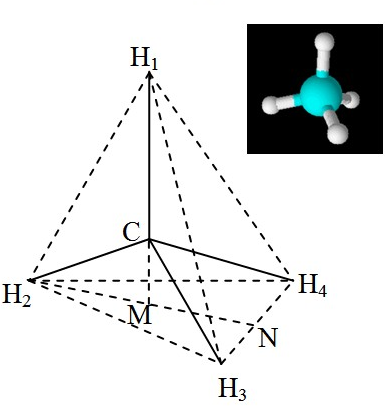
\includegraphics[width=3.35in,height=2.5in,viewport=14 14 250 190,clip]{Tetrahedron.eps}
\caption{\small Arrangement of the secant plane of constant energy in the method of tetrahedrons when $E_0\leqslant E\leqslant E_1$.}
\label{Tetrahedron}
\end{figure}

态密度的一般表达式为,
\begin{equation}
  N_A(E)=\frac1N\sum_{\vec k}A(\vec k)\delta(E-E(\vec k))=\frac{dD_A(E)}{dE}
  \label{eq:solid-198}
\end{equation}
这里
\begin{equation}
  D_A(E)=\frac1N\sum_{\vec k}A(\vec k)\theta(E-E(\vec k))
  \label{eq:solid-199}
\end{equation}
这里$\theta(x)$是Heavyside阶梯函数;$A(\vec k)$是关于矢量$\vec k$的任意函数。对应于式\eqref{eq:solid-197}的三种情况,
电子态密度的表达式分别为,
\begin{enumerate}
\item $E_0\leqslant E\leqslant E_1$
\begin{equation}
  \begin{split}
    N_A(E)=&\frac{|\vec k_{10}[\vec k_{20}\cdot\vec k_{30}]|}\Omega_0\frac{(E-E_0)^2/2}{(E_1-E_0)(E_2-E_0)(E_3-E_0)}\\
    &\cdot\left\{A_0+\left[\frac{A_1-A_0}{E_1-E_0}+\frac{A_2-A_0}{E_2-E_0}+\frac{A_3-A_0}{E_3-E_0}\right](E-E_0)/3\right\}
  \end{split}
  \label{eq:solid-200}
\end{equation}
\item $E_1\leqslant E\leqslant E_2$
\begin{equation}
  \begin{split}
    N_A(E)=&\frac{|\vec k_{10}[\vec k_{20}\cdot\vec k_{30}]|}\Omega_0\left\{\frac{(E-E_0)^2/2}{(E_1-E_0)(E_2-E_0)(E_3-E_0)}\right.\\
    &\cdot\left[A_0+\left(\frac{A_1-A_0}{E_1-E_0}+\frac{A_2-A_0}{E_2-E_0}+\frac{A_3-A_0}{E_3-E_0}\right)(E_3-E_0)/3\right]\\
    &-\frac{(E-E_1)^2/2}{(E_1-E_0)(E_2-E_1)(E_3-E_1)}\\
    &\cdot\left.\left[A_1+\left(\frac{A_1-A_0}{E_1-E_0}+\frac{A_2-A_1}{E_2-E_1}+\frac{A_3-A_1}{E_3-E_1}\right)\frac{(E-E_1)}3\right]\right\}
  \end{split}
  \label{eq:solid-201}
\end{equation}
\item $E_2\leqslant E\leqslant E_3$
\begin{equation}
  \begin{split}
    N_A(E)=&\frac{|\vec k_{10}[\vec k_{20}\cdot\vec k_{30}]|}\Omega_0\frac{(E_3-E)^2/2}{(E_3-E_0)(E_3-E_1)(E_3-E_2)}\\
    &\cdot\left\{A_3-\left[\frac{A_3-A_0}{E_3-E_0}+\frac{A_3-A_1}{E_3-E_1}+\frac{A_3-A_2}{E_3-E_2}\right](E_3-E)/3\right\}
  \end{split}
  \label{eq:solid-202}
\end{equation}
\end{enumerate}

%二次插值方法选择一个大的立方体,%作为工作体积,
%将该立方体分割为小的立方体,立方体的数目为$M^3$,这里$M$取决于计算要求的精度。用通过小立方体体心的三个剖面将每个小立方体分割出27个等价点,$\vec k$点的能量本征值$E(\vec k)$由27个点确定,$E(\vec k)$用小立方体内的一系列$\vec k$点展开到二阶,
%\begin{equation}
%  E(\vec k)=E_0+\vec m\vec k+\vec k\mathbf Q\vec k=\sum_{i=1}^{10}A_ia_i(\vec k)
%  \label{eq:solid-203}
%\end{equation}
%这里$A_i$是展开系数;$a_i(\vec k)$是$\vec k_x$,$\vec k_y$,$\vec k_z$的线性组合到二阶。
晶体的$\vec k$空间积分,除了四面体线性插值外,过去二次插值也是用得比较多的积分方法。关于二次插值的详细介绍,可以参考文献\cite{AP67-15_1971}。无论是线性插值还是二次插值,都各有优劣。对过渡金属,由于其复杂的能带结构,需要很多临界点(高对称性点)的解析解,而且体系的态密度主要由临界点决定,因此对临界点需要高精度的解析计算,但是用线性插值方法很难得到。但是四面体线性插值可以使得整个\textrm{Brillouin}区积分解析完成,因此提高了Fermi能级和Fermi面附近的态密度的计算精度,而这对于金属和导体计算非常重要。此外,线性插值方法也有助于处理非解析临界点(能带交叉点)的情况\cite{PLA28-570_1969,PRB7-891_1973,PRB5-1276_1972}。

能带交叉是\textrm{Brillouin}区积分误差的重要来源,在Brillouin区中接近交叉点的小区域内$|\nabla_{\vec k}E(\vec k)|\simeq0$,会导致$N(E)$的能量奇点的出现,以致于出现不正确的插值计算。%伴随能带交叉产生的另外一个问题是交叉点附近不同可观测物理量的矩阵元的行为。
能带交叉导致矩阵元在交叉点变化剧烈,如果插值点位于这些交叉点上,可能引起更大的误差。理论上,计算精度可以通过增加线性插值的四面体数目%或者二次插值中的参数$M$
来提高,因此插值方法的计算精度主要由布点数目决定。

%有时常将两种方法结合使用,用二次插值计算各参考点的线性插值部分,然后用线性四面体方法计算积分。与之类似的思想就是混合插值,用二次插值得到式\eqref{eq:solid-194}中的梯度
%\begin{equation}
%  \nabla E(\vec k)=\sum_{i=1}^{10}A_i\nabla C_i(\vec k)
%  \label{eq:solid-204}
%\end{equation}
%这里$C_i(\vec k)$式$k_x$,$k_y$,$k_z$的简单解析函数。

\subsection{改进的四面体方法与误差修正}\label{New_Tetrahedron}
四面体方法是更普适的一般方法,除了可用于绝缘体、半导体、金属的期望值计算,还可以计算体系的谱函数,即体系的动态响应性质。但是传统的四面体插值方法为了减少统计四面体的数目,选择在不可约\textrm{Brillouin}区内分割四面体,但这一策略有副作用,由于不可约部分的不规则性,其中的四面体划分几乎不可避免地要人工干预,因此生成四面体的程序化非常困难,\textrm{Bl\"ochl}等改进了线性四面体插值积分方法\cite{PRB49-16223_1994},提出了在已知空间群的情况下,用不可约$\vec k$点快速自动生成四面体的方案,避免了传统方法中分割四面体复杂过程:~
\begin{enumerate}
	\item 利用\textrm{Monkhorst-Pack}方案\cite{PRB13-5188_1976}首先在第一\textrm{Brillouin-zone}内生成等体积的平行六面体网格,并依次用式\eqref{eq:kpoint_Tetra-blochl}的值给每个网格点编号:
\begin{equation}
	N=1+\dfrac{i-i_0}2+(n_1+1)\left[\dfrac{j-j_0}2+(n_2+1)\dfrac{k-k_0}2\right]
	\label{eq:kpoint_Tetra-blochl}
\end{equation}
这里$i,j,k$分别是该$\vec k$点沿倒格矢$\mathbf{b}_i(i=1,2,3)$的序数的二倍,$i_0,j_0,k_0$是\textrm{Monkhorst-Pack}方法中$\Gamma$点许可的偏移量,有偏移则为1,否则为0
	\item 编号之后建立$\vec k$点标识数组,其位置与该位置储存的元素编号值相同,例如,第一个位置存储“$1$”,第二个位置存储“$2$”,依次类推;~
	\item 从第一个位置开始,利用点群的操作元素作用于每个$\vec k$点坐标,并与数组中其余$\vec k$点的坐标进行比较,如果彼此相同且后者的编号大于前者,即将后者的元素编号值改为前者(遍历全部$\vec k$点,可以挑出所有不可约$\vec k$~点:~并且只有当$\vec k_i$为不可约$\vec k$~点时,其编号才与其存储位置相同)。
	\item 为了计算方便,对所有这些不可约$\vec k$点按存储位置的顺序重新编号,即从“$1$”到“$\vec k_{\mathrm{irr}}(\max)$”。并将整个第一\textrm{Brillouin-zone}中的点都用对应的等价不可约点的编号值标记。
	\item 平行六面体中的四面体的自动划分:~
		\begin{itemize}
			\item 假设以下八组坐标代表的点构成平行六面体:
\begin{displaymath}
	\begin{aligned}
		&(l,m,n)\rightarrow 1,&(l+1,m,n)\rightarrow 2\\
		&(l,m+1,n)\rightarrow 3,&(l+1,m+1,n)\rightarrow 4\\
		&(l,m,n+1)\rightarrow 5,&(l+1,m,n+1)\rightarrow 6\\
		&(l,m+1,n+1)\rightarrow 7,&(l+1,m+1,n+1)\rightarrow 8
	\end{aligned}
\end{displaymath}
为了尽量减小插值引起的误差,可以取此平行六面体中最短的体对角线作为等体积的六个四面体的公共对角线,设为$3-6$(图\ref{Fig:Submesh_Tetra}),则可以采用下面6组途径确定这六个四面体的各个顶点:~
\begin{displaymath}
	\begin{aligned}
		1\rightarrow2\rightarrow3\rightarrow6\quad&1\rightarrow3\rightarrow5\rightarrow6\quad&2\rightarrow3\rightarrow4\rightarrow6\\
		3\rightarrow5\rightarrow6\rightarrow7\quad&3\rightarrow4\rightarrow6\rightarrow8\quad&3\rightarrow6\rightarrow7\rightarrow8
	\end{aligned}
\end{displaymath}
		\end{itemize}
\begin{figure}[h!]
\centering
\vspace*{-0.28in}
\includegraphics[height=1.25in,width=3.00in,viewport=0 0 1350 705,clip]{submesh_Tetra.png}
\caption{\small Breakup of a submesh cell into six tetrahedra.}%(与文献\cite{EPJB33-47_2003}图1对比)
\label{Fig:Submesh_Tetra}
\end{figure}
	\item 对每个平行六面体重复上述过程,将第一\textrm{Brillouin-zone}划分为体积相等的若干四面体,每个四面体的顶点可用标识数组中的不可约点编号值标记。
	\item 将每个四面体的四个顶点按编号值升序排列,可以方便地确定等价四面体(顶点编号完全相同的四面体,即为等价四面体)。
\end{enumerate}

这个过程保证了只用不可约点上的信息进行整个第一\textrm{Brillouin}区分割,无须考虑如何划定其不可约部分,
%上述过程可以避免Kleinman所说的计算误差,而且整个过程可以通过程序自动实现而无须人工干预。上述过程可以避免计算误差,
而且整个过程可以通过程序自动实现,无须人工干预。

%仿照特殊点方法,将积分变成不可约$\vec k$点的积分权重求和,
%\begin{equation}
%  \langle X\rangle=\frac1{\Omega_0}\sum_n\int_{\Omega_0}d^3kX_n(\vec k)f(\varepsilon_n(\vec k))=\sum_{jn}X_n(\vec k_j)w_{nj}
%  \label{eq:solid-207}
%\end{equation}
%这里$X_n(\vec k_j)$是可观测量$\langle X\rangle$在不可约$\vec k$点的矩阵元:$X_n(\vec k)=\langle\Psi_n(\vec k)|X|\Psi_n(\vec k)\rangle$;
Brillouin区中任意一点$\vec k$的函数值$X_n(\vec k)$可以通过四面体线性插值得到,
\begin{equation}
  X_n(\vec k)=\sum_jX_n(\vec k_j)w_j(\vec k)
  \label{eq:solid-208}
\end{equation}
$w_j(\vec k)$是四面体插值权重,当积分点在不可约点$\vec k_j$(或者其等价点)上时,插值权重为1,其余不可约点权重为零;在四面体内部,插值权重为线性函数,权重的定义为:
\begin{equation}
	w_{nj}(\vec k)=\frac1{\Omega_0}\int_{\Omega_0}d^3\vec kw_j(\vec k)f(\varepsilon_n(\vec k))
	\label{eq:solid-209}
\end{equation}
对于给定的能带,四面体方法的积分权重也只需计算一次。

\textrm{Bl\"ochl}等在改进四面体方法中专门考虑的积分误差的问题,由此导出了四面体方法对导体和金属积分的修正公式。四面体积分的误差主要有两个来源(如图\ref{Fig:Tetra_error}所示):
	\begin{enumerate}
		\item 四面体内的线性插值引起的误差;~
		\item 临近真实\textrm{Fermi~}面时,四面体内等能面线性插值逼近引入的误差。
	\end{enumerate}
\begin{figure}[h!]
\centering
\vspace*{-0.28in}
\includegraphics[height=1.25in,width=1.25in,viewport=0 0 650 650,clip]{Tetra_error.png}
\caption{\small Schematic representation of the interpolation error due to line interpolation.}%(与文献\cite{EPJB33-47_2003}图1对比)
\label{Fig:Tetra_error}
\end{figure}

对半导体和绝缘体,由于价带被完全填充,通过\textrm{Monkhorst-Pack}布点产生四面体布点方案,只要$\vec k$点足够密集,可以保证在临近\textrm{Fermi}面的线性插值误差完全抵消;~对导体和金属,每个四面体内的线性插值积分误差
\begin{equation}
	\delta\langle X\rangle_T=\int_T\mathrm{d}^3k\left[ X(\vec k)-\bar X(\vec k) \right]
  	\label{eq:solid-Tetra_metal}
\end{equation}
为估计积分误差,假设有被积函数
$$X(\vec k)=a+\sum_ib_ik_i+\frac12\sum_{ij}k_ic_{ij}k_j$$
如果四面体的一个顶点置于原点,其余三个点位于$\vec t_i=(t_{1i},t_{2i},t_{3i})$%(如图\ref{Fig:Tetrahedron}),其中
$i=1,2,3$
%\begin{figure}[h!]
%\centering
%\vspace*{-0.3in}
%\includegraphics[height=1.65in,width=1.70in,viewport=15 15 500 550,clip]{Brillouin-Tetra.eps}
%\caption{\small .}%(与文献\cite{EPJB33-47_2003}图1对比)
%\label{Fig:Tetrahedron}
%\end{figure}
将坐标系$s_i$作线性变换,
$$k_i=\sum_jt_{ij}s_j$$
因此被积函数变换为
$$X(\vec s)=\bar a+\sum_i\bar b_is_i+\frac12\sum_{ij}s_i\bar c_{ij}s_j$$
这里系数$\bar a=a$,$\bar b_i=\sum\limits_jb_jt_{ji}$,$\bar c_{ij}=\sum\limits_{kl}t_{kl}c_{kl}t_{lj}$\\
并且$s_i>0\;i=1,2,3$,$\sum\limits_{i=1}^3s_i\leqslant1$
于是被积函数的线性插的近似值为
$$\bar X(\vec s)=\bar a+\sum_i(\bar b_i+\frac12\bar c_{ii})s_i$$
因此可有积分误差的解析表示为
	\begin{displaymath}
		\begin{aligned}
			\delta\langle X\rangle_T=&\mathrm{det}|t_{ij}|\int_T\mathrm{d}^3s\frac12\left[ \sum_{ij}s_i\bar c_{ij}s_j-\sum_i\bar c_{ii}s_i \right]\\
			=&\frac16\mathrm{det}|t_{ij}|\frac1{40}\left[ \sum_{i\neq j}\bar c_{ij}-3\sum_i\bar c_{ii} \right]
		\end{aligned}
	\end{displaymath}
将$c_{ij}$用被积函数的二阶导数表示,$\frac16\mathrm{det}|t_{ij}|$是四面体体积$V_T$,因此可有
	\begin{displaymath}
		\delta\langle X\rangle_T=V_T\sum_{ij}\left\langle\frac{\partial^2X}{\partial k_i\partial k_j}\right\rangle_TC_{ii}\Delta^2
	\end{displaymath}
这里$\Delta=\sqrt[3]{\mathrm{det}|t|}$
	$$C_{ij}=\frac1{40\Delta^2}\left[ \sum_{l\neq m}t_{il}t_{jm}-3\sum_lt_{ij}t_{jl} \right]$$

对全部占据四面体误差$\delta\langle X\rangle_T$求和,得到插值误差
	\begin{equation}
		\delta\langle X\rangle=\left\langle\sum_{ij}\frac{\partial^2X}{\partial k_i\partial k_j}C_{ii}\right\rangle\Delta^2
		\label{eq:kpoint_Tetra_error}
	\end{equation}
所以四面体积分的误差随$\Delta^2$收敛。

根据\textrm{Green's}积分公式,可将体相积分变成\textrm{Fermi}面的表面积分
	\begin{equation}
		\begin{aligned}
			\delta\langle X\rangle=&\frac1{V_G}\sum_{ij}\langle C_{ij}\rangle\int_{V_G}\mathrm{d}^3k\frac{\partial^2X}{\partial k_i\partial k_j}\Delta^2\\
			=&\frac1{V_G}\sum_{ij}\langle C_{ij}\rangle\oint_{\varepsilon=\varepsilon_{\mathrm F}}\mathrm{d}^2A_i\frac{\partial X}{\partial k_j}\Delta^2
		\end{aligned}
		\label{eq:kpoint_Tetra_surface}
	\end{equation}
因此可有
	\begin{displaymath}
			\delta\langle X\rangle=\frac1{V_G}\sum_{ij}\oint_{\varepsilon=\varepsilon_{\mathrm F}}\mathrm{d}^2A_iC_{ij}\frac{\partial X}{\partial k_j}\Delta^2
	\end{displaymath}
将如下等式
	\begin{displaymath}
		\begin{aligned}
		&\int\mathrm{d}^2A_i=\int\mathrm{d}^2|A|\frac1{\nabla_k\varepsilon}\frac{\partial\varepsilon}{\partial k_i}\\
		&\sum_i\frac{\partial\varepsilon}{\partial k_i}t_{ij}=\varepsilon_{j+1}-\varepsilon_1\\
		&\sum_i\frac{\partial X}{\partial k_i}t_{ij}=X_{j+1}-X_1 
		\end{aligned}
	\end{displaymath}
这里$\varepsilon_i$和$X_i$是四面体顶点的能量和被积函数值,代入最终得到的四面体积分误差校正公式为:~
\begin{equation}
	\begin{aligned}
		\delta\langle X\rangle=&\sum_TD_T(\varepsilon_{\mathrm F})\frac1{40}\left[\sum_{i\neq j}(X_{i+1}-X_1)(\varepsilon_{j+1}-\varepsilon_1)\right.\\
			&-3\left.\sum_i(X_{i+1}-X_1)(\varepsilon_{j+1}-\varepsilon_1)\right]\\
			=&\sum_TD_T(\varepsilon_{\mathrm F})\frac1{40}\sum_{i=1}^4X_i\sum_{j=1}^4(\varepsilon_j-\varepsilon_i) 
	\end{aligned}
	\label{eq:kpoint_Tetra_blochl-error}
\end{equation}
相应地,积分权重校正公式为
\begin{equation}
	\mathrm{d}w_i=\frac{\delta\langle X\rangle}{\delta X_i}=\sum_T\frac1{40}D_T(\varepsilon_{\mathrm F})\sum_{j=1}^4(\varepsilon_j-\varepsilon_i) 
	\label{eq:kpoint_Tetra_blochl-weighterror}
\end{equation}

类似地,考虑等能面线性插值对\textrm{Fermi~}面逼近引起的误差,可有每个四面体的电子数校正:~
\begin{displaymath}
	\delta N_{\mathrm{el},T}=\frac{A_T}{V_G}\sum_{ij}\frac{\partial^2k_{\mathrm F}}{\partial k_i\partial k_j}C_{ij}\Delta^2
\end{displaymath}
这里$A_T$是三角形面积,三角形的形状因子$C_{ij}$表达式为:~
$$C_{ij}=\frac1{24\Delta^2}\left[ \sum_{l\neq m}t_{il}t_{jm}-2\sum_lt_{ij}t_{jl} \right]$$
其中$t_{ij}$是与四面体类似的三角形顶点矢量。%对均匀电子分布,四面体积分误差随$\Delta^3$收敛

%对于导体和金属,传统四面体方法在计算\textrm{Fermi}面附近积分时,都会引入展宽
%四面体积分$W=\dfrac{\mathrm{d}w_i}{\mathrm{d}\varepsilon}$对能量导数对应于“展宽”
%\begin{figure}[h!]
%\centering
%\vspace*{-0.28in}
%\includegraphics[height=1.4in,width=1.55in,viewport=0 0 1000 800,clip]{Tetra_smearing.png}
%%\caption{\small .}%(与文献\cite{EPJB33-47_2003}图1对比)
%\label{Fig:Tetrahedron}
%\ end{figure}
%\begin{itemize}
%\vspace*{-0.1in}
%	\item \textcolor{blue}{四面体方法展宽参数可随能带分布和形状\\
% 	传统展宽方法的展宽系数对所有能带都相同}
% 	\item \textcolor{red}{四面体方法不推荐引入展宽参数}\\
%		\begin{enumerate}
%			\item 展宽计算的总能不满足变分原理,\textrm{Hellmann-Feynman}定理不再满足,\textcolor{red}{不能正确计算导体的受力}
%			\item 四面体能保证态密度计算在\textrm{van Hove}奇点附近出现振荡,引入展宽会破坏这一特征
%		\end{enumerate}
%\end{itemize}

%针对改进后的四面体方法,\textrm{Bl\"ochl}提出了一个形式简单的积分校正公式,
%\begin{equation}
%  \delta\langle X\rangle=\sum_TD_T(\varepsilon_F)\frac1{40}\sum_{j=1}^4X_i\sum_{j=1}^4(\varepsilon_F-\varepsilon_i)
%  \label{eq:solid-205}
%\end{equation}
%相应的积分权重校正为:
%\begin{equation}
%  dw_i=\frac{d\langle X\rangle}{d X_i}=\sum_T\frac1{40}D_T{\varepsilon_F}\sum_{j=1}^4(\varepsilon_F-\varepsilon_i)
%  \label{eq:solid-206}
%\end{equation}
%可以很好的提高对金属的计算结果,而对绝缘体,用改进四面体积分方法用同等数量的布点,可以得到与特殊点方法相同的结果。

%\subsection{晶体的总能量}
%晶体总能量(不包括核的动能)可以分为两部分:一部分是原子核与芯电子组成的离子实能量,这部分能量基本上与晶体结构($\{\vec R\}$)无关,是一个常数,约为$-$$10^3$\,Ry/原子(在固体物理中讨论能量一般沿用Ry单位);另一部分是总能与离子实之差,即离子与价电子的相互作用、离子间的相互作用以及价电子间相互作用,约为$-$10\,Ry/原子。赝势(Pseudo Potential, PP)方法中常把总能量中不变的常数部分(即离子实的能量)设为零。晶体的结合能定义为这部分总能加上核的动能(通常是零点振动能)与孤立原子的能量差。在密度泛函理论中,赝势方法的晶体总能量$E_T$是晶格电子能量$E_{e\textrm{-}e}$与离子实排斥能$E_{N\textrm{-}N}$之和:
%\begin{equation}
%  E_T=E_{e\textrm{-}e}+E_{N\textrm{-}N}=T[\rho]+E_{ext}+E_{Coul}+E_{xc}+E_{N\textrm{-}N}
%  \label{eq:solid-total}
%\end{equation}
%根据Kohn-Sham方程%\eqref{eq:dft-10}
%,动能泛函用单电子能量表示为
%\begin{equation}
%  T[\rho]=\sum_i\langle\psi_i|E_i-V_{KS}|\psi\rangle
%  \label{eq:solid-49}
%\end{equation}
%于是可以得到
%\begin{equation}
%  E_T=\sum_i\varepsilon_i-\frac12\iint d\vec rd\vec r'\dfrac{\rho(\vec r)\rho(\vec r')}{|\vec r-\vec r'|}+\int d\vec r\rho(\vec r)[\varepsilon_{xc}(\vec r)-V_{xc}(\vec r)]+E_{N\textrm{-}N}
%  \label{eq:solid-50}
%\end{equation}
%在计算晶体总能量时,如果利用晶格的周期性,将实空间($\vec r$空间)总能量表示转换到动量空间($\vec k$空间)将使得计算十分便利。
%\begin{equation}
%  E_T=\sum_i\varepsilon_i-\frac{\Omega_0}2\sum_{\vec k\neq0}\rho^{\ast}(\vec k)V_{Coul}(\vec k)+\Omega_0\sum_{\vec k}\rho^{\ast}(\vec k)[\varepsilon_{xc}(\vec k)-V_{xc}(\vec k)]+E_{N\textrm{-}N}
%  \label{eq:solid-51}
%\end{equation}
%这里$V_{Coul}(\vec k)$,$\varepsilon_{xc}(\vec k)$,$V_{xc}(\vec k)$和$\rho(\vec k)$分别是电子间Coulomb相互作用势、电子交换-相关能、交换-相关势和电子密度的Fourier分量,$\Omega_0$为原胞体积。其中电子间Coulomb势的Fourier分量$V_{Coul}(\vec k)$可以从Poisson方程
%\begin{equation}
%  \nabla^2V_{Coul}(\vec r)=-8\pi\rho(\vec r)
%  \label{eq:poisson-r}
%\end{equation}
%用Fourier展开得到
%\begin{equation}
%  V_{Coul}(\vec k)=\dfrac{8\pi\rho(\vec k)}{k^2}
%  \label{eq:poisson-k}
%\end{equation}
%对于交换-相关能和交换相关势,一般根据交换-相关能近似在实空间求得的$\varepsilon_{xc}(\vec r)$和$V_{xc}(\vec r)$后,用Fourier变换到动量空间,得到$\varepsilon_{xc}(\vec k)$和$V_{xc}(\vec k)$。
%
%在实际计算中,需要必要的数学处理,因为离子间Coulomb相互作用能之和:
%$$E_{N\textrm{-}N}=\dfrac12\sum_{\vec r,s}\sideset{}{'}\sum_{\vec R',s'}\dfrac{Z_sZ_{s'}}{|\vec R+\vec{\tau}_s-\vec R'-\vec{\tau}_{s'}|}$$
%这里$Z_s$表示价电子数,$\vec R$表示晶格的格式,$\tau$表示原胞内的原子相对位矢。其求和包含无穷多项;此外$V_{Coul}(\vec k=0)$是发散的;而$V_{ext}$在不考虑其他外场,一般只考虑离子与电子的Coulomb相互作用,
%\begin{equation}
%  \begin{split}
%    V_{ext}(\vec r)=&\sum_{\vec r,s}\dfrac{-2Z_s}{|\vec r-\vec R-\vec r_s|}=\sum_{\vec r,s}\dfrac{-2Z_s}{|\vec r-\vec R-\vec{\tau}_s|} \\
%    =&\sum_{\vec r,s}v_{ext}'(\vec r-\vec R-\vec{\tau}_s)
%  \end{split}
%  \label{eq:solid-52}
%\end{equation}
%它的Fourier分量在$\vec k=0$也是发散的。由于这三项单独都是发散的,但因为整个系统处于电中性,这些发散项相互抵消,是一个常数。因此在解Kohn-Sham方程的时候,可先将$V_{Coul}(\vec k=0)$和$V_{ext}(\vec k=0)$同时置为零,这相当于将势能作一平移,或者说重新定义真空能级,而在总能量计算中补偿这一平移。记这些发散项的和为:
%\begin{equation}
%  \begin{split}
%    \lim\limits_{\vec k\rightarrow0}&\Omega_0\left[\dfrac12V_{Coul}(\vec k)+\sum_sv_{ext}^s(\vec k)\right]\rho(\vec k)+\dfrac12\sum_{\vec R,s}\sideset{}{'}\sum_{\vec R',s'}\dfrac{2Z_sZ_{s'}}{|\vec R+\vec{\tau}_s-\vec R'-\vec{\tau}_{s'}|} \\
%    &=\sum_s\alpha_s\sum_sZ_s+E_{Ewald}
%  \end{split}
%  \label{eq:solid-53}
%\end{equation}
%
%对于形如$Z_s/r$的外场,它的Fourier分量在$\vec k=0$附近展开:$v_{ext}^s(\vec k)=-\dfrac{8\pi Z_s}{\Omega_0k^2}+\alpha_s+o(\vec k)$,同样的展开$\rho(\vec k)$,有$\lim\limits_{\vec k\rightarrow0}\rho(\vec k)=\dfrac{\sum\limits_sZ_s}{\Omega_0}+\beta k^2+o(\vec k)$,代入式\eqref{eq:solid-53},去掉$\vec k$的高次项,有
%\begin{equation}
%  \begin{split}
%    \lim\limits_{\vec k\rightarrow0}&\biggl[\dfrac{\Omega_0}2\dfrac{8\pi\rho^2(\vec k)}{k^2}+\Omega_0\left(\dfrac{-8\pi\sum\limits_sZ_s}{\Omega_0k^2}+\sum_s\alpha_s\right)\rho(\vec k)+\frac12\dfrac{8\pi(\sum\limits_sZ_s)^2}{\Omega_0k^2}\biggr]\\
%    &+\frac12\sum_{\vec R,s}\sideset{}{'}\sum_{\vec R',s'}\dfrac{2Z_sZ_{s'}}{|\vec R+\vec{\tau}_s-\vec R'-\vec{\tau}_{s'}|}-\lim\limits_{\vec k\rightarrow0}\frac12\dfrac{8\pi(\sum\limits_sZ_s)^2}{\Omega_0k^2}\\
%    =&\sum_s\alpha_s\sum_sZ_s+E_{Ewald}
%  \end{split}
%  \label{eq:solid-54}
%\end{equation}
%其中离子间排斥能可用Ewald方法得到\cite{Born-Huang}:
%\begin{equation}
%  \begin{split}
%    E_{Ewald}=&\frac12\sum_{\vec R,s}\sideset{}{'}\sum_{\vec R',s'}\dfrac{2Z_sZ_{s'}}{|\vec R+\vec{\tau}_s-\vec R'-\vec{\tau}_{s'}|}-\lim\limits_{\vec k\rightarrow0}\frac12\dfrac{8\pi(\sum\limits_sZ_s)^2}{\Omega_0k^2} \\
%    =&\frac12\sum_{\vec R,s}\sideset{}{'}\sum_{\vec R',s'}\dfrac{2Z_sZ_{s'}}{|\vec R+\vec{\tau}_s-\vec R'-\vec{\tau}_{s'}|}-\frac1{\Omega_0}\sum_{s,s'}\int d\vec r\frac{Z_sZ_{s'}}r \\
%    =&\sum_{s,s'}Z_sZ_{s'}\left\{\frac{4\pi}{\Omega_0}\sum_{\vec k\neq0}\cos[\vec k\cdot(\vec{\tau}_s-\vec{\tau}_{s'})]\dfrac{e^{-k^2/4\eta^2}}{k^2}\right.\\
%    &-\left.\frac{\pi}{\eta^2\Omega_0}+\frac12\sum_{\vec r}\left.\dfrac{erf(\eta x)}x\right|_{\vec R+\vec{\tau}_s-\vec{\tau}_{s'}\neq0}-\dfrac{2\eta}{\sqrt{\pi}}\delta_{s,s'}\right\}
%  \end{split}
%  \label{eq:solid-55}
%\end{equation}
%这里$erf(x)$是误差函数,参数$\eta$原则上是任意的,如果$\vec r$取得足够多,上述求和是与$\eta$无关的。一般选取$\eta$使得在正格子和倒格子空间收敛得足够快。而$\alpha_s$可根据实际的$v_{ext}^s(\vec r)$得到:
%\begin{equation}
%  \alpha_s=\lim\limits_{\vec k\rightarrow0}\left[v_{ext}^s(\vec k)+\dfrac{8\pi Z_s}{\Omega_0k^2}\right]=\dfrac1{\Omega_0}\int d\vec r\left[v_{ext}^s(\vec r)+\dfrac{2Z_s}r\right]
%  \label{eq:solid-56}
%\end{equation}
%由此得到总能量
%\begin{equation}
%  \begin{split}
%   E_T=&\sum_i\varepsilon_i-\dfrac{\Omega_0}2\sum_{\vec k\neq0}\rho^{\ast}(\vec k)V_{Coul}(\vec k)+\Omega_0\sum_{\vec k}\rho^{\ast}(\vec k)[\varepsilon_{xc}(\vec k)-V_{xc}(\vec k)]\\
%   &+\sum_s\alpha_s\sum_sZ_s+E_{Ewald}
%  \label{eq:solid-57}
%  \end{split}
%\end{equation}
%
%全势方法同样改进了求解Madelung势能的计算方法\cite{JMP22-2433_1981}。MT近似下,WS原胞内中MT球的球心位于$\vec\gamma_{\nu}$,$R_{\nu}$为半径。如果球面上的势能平均为$S_0(R)$,除去球心核电荷以外所有电荷在MT球面上产生的势能平均为:
%\begin{equation}
%  S(R_{\nu})\equiv S_0(R_{\nu})+Z_{\nu}/R_{\nu}
%  \label{eq:solid-79}
%\end{equation}
%则根据$S(R_{\nu})$和球形Dirichlet边值问题\cite{JMP22-2433_1981},球心$\vec\gamma_{\nu}$处的Madelung势(因为要求的Madelung势位于球心,只有$l=0$部分对此有贡献,故只需考虑$S(R_{\nu})$的球形平均部分)为\cite{PRB26-4571_1982}:
%\begin{equation}
%  \begin{split}
%   V_M(\vec\gamma_{\nu})&=\frac1{R_{\nu}}[R_{\nu}S_0(R_{\nu})+Z_{\nu}-Q_{\nu}]+\sqrt{4\pi}\int_0^{R_{\nu}}drr\rho_{00}(r_{\nu})\\
%   &=\frac1{R_{\nu}}[R_{\nu}S_0(R_{\nu})+Z_{\nu}-Q_{\nu}]+\bigg\langle\frac1r\rho(\vec r)\bigg\rangle_{\nu}
%  \end{split}
%   \label{eq:Madelung}
%\end{equation}
%其中$Q_{\nu}$表示MT球内的电子电荷之和。$\rho(\vec r)$是MT球内的电荷密度,可以用球谐函数表示为
%\begin{equation}
%  \rho(\vec r_{\nu})=\sum_{lm}\rho_{lm}(r_{\nu})Y_{lm}(\hat r_{\nu})
%  \label{eq:solid-80}
%\end{equation}
%类似地,WS原胞内的总能量可以表示为:
%\begin{equation}
%  \begin{split}
%   E_T=&\sum_i\varepsilon_i-\frac12\int_{\Omega_0}\rho(\vec r)[V_c(\vec r)+2\mu_{xc}(\vec r)]d\vec r-\frac12\sum_{\nu}Z_{\nu}V_M(\vec\gamma_{\nu})+E_{xc}[\rho] \\
%   =&\sum_i\varepsilon_i-\frac12\left(\int_{\Omega_0}\rho(\vec r)V_c(\vec r)d\vec r+\sum_{\nu}Z_{\nu}\bigg\langle\frac1r\rho(\vec r)\bigg\rangle_{\nu}\right)-\int_{\Omega_0}\rho(\vec r)\mu_{xc}(\vec r)d\vec r\\
%   &-\frac12\sum_{\nu}\frac{Z_{\nu}}{R_{\nu}}[R_{\nu}S_0(R_{\nu})+Z_{\nu}-Q_{\nu}]+E_{xc}[\rho]
%  \end{split}
%  \label{eq:solid-81}
%\end{equation}
%这里$V_c(\vec r)=\int\dfrac{\rho(\vec r')}{|\vec e-\vec r'|}d\vec r'-\sum\limits_{\alpha}\dfrac{Z_{\alpha}}{|\vec r-\vec r_{\alpha}|}$。总能量写成这样的形式,原子核位置的Coulomb势奇点可以排除。将势能和电荷密度在各原子核附近作球谐展开,在原子核附近,有
%\begin{displaymath}
%  \begin{split}
%    &\int_{\Omega_0}\rho(\vec r)V_c(\vec r)d\vec r+Z{\nu}\sqrt{4\pi}\int_0^{R_{\nu}}drr^2\frac{\rho_{00}(r)}r\\
%    =&\sqrt{4\pi}\int_{\Omega_0}drr^2\rho_{00}(\vec r)\left(V_{00}(r)Y_{00}(\hat r)+\frac{Z_{\nu}}r\right)+\sum_{lm>0}\int drr^2\rho_{lm}(r)V_{lm}(r)
%  \end{split}
%\end{displaymath}
%Coulomb势的奇点只出现在$V_{00}(r)$中,将$V_{00}(r)$写成核的点电荷势与源于电子的平滑势两部分之和,有
%$$V_{00}(r)=-\sqrt{4\pi}\frac{Z_{\nu}}r+\hat V_{00}(r)$$
%有必要指出的是,通过这样的方式,可以将总能量中的奇点排除,但是单独每一项在原子核位置能量仍然是发散的。
%
%如果采用标准的LDA近似,式\eqref{eq:solid-81}交换-相关能可以写成:
%\begin{equation}
%  E_{xc}[\rho]\approx\int_{\Omega_0}\rho(\vec r)\varepsilon_{xc}(\vec r)d\vec r
%  \label{eq:solid-82}
%\end{equation}
%
%一般地,总能量计算在动量空间中完成。在MT近似下,间隙区的电荷密度用平面展开,有
%$$\rho(\vec r)=\sum_{\vec G}e^{i\vec G\cdot\vec r},\quad \vec r\in\mathrm{Interstitial}$$
%在MT球内,电荷密度用球谐函数展开,在动量空间中的展开形式为:
%$$\bar\rho_{lm}(r_{\nu})=4\pi i^l\sum_{\vec G}\rho(\vec G)e^{i\vec G\cdot\vec{\gamma}_{\nu}}j_l(Gr_{\nu})Y_{lm}^{\ast}(\vec G)$$
%于是,WS原胞内的晶体总能量可以写成:
%\begin{equation}
%  \begin{split}
%  E=&\sum_i\varepsilon_i-\sum_{\vec G}\Omega_0\rho(\vec G)-\frac12\sum_{\nu}\dfrac{Z_{\nu}}{R_{\nu}}[Z_{\nu}-Q_{\nu}+R_{\nu}S_0(R_{\nu})]\\
%  &-\sum_{\nu}\sum_{lm}\int_0^{R_{\nu}}drr^2\left[\rho_{lm}(r_{\nu})\left(\tilde V_{lm}^{\ast}(r_{\nu})\dfrac{\sqrt{4\pi}}{2r_{\nu}}Z_{\nu}\delta_{l0}\right)-\bar\rho_{lm}(\vec r_{\nu})\bar V_{lm}^{\ast}(\vec r_{\nu})\right]
%  \end{split}
%  \label{eq:solid-83}
%\end{equation}
%这里$\tilde V(\vec r)$和$\bar V_{lm}(\vec r)$根据下式计算:
%$$\tilde V(\vec r)=\frac12V_c(\vec r)-\varepsilon_{xc}(\vec r)+\mu_{xc}(\vec r)$$
